% Previous Work Section

\begin{figure*}[!t]
\centering
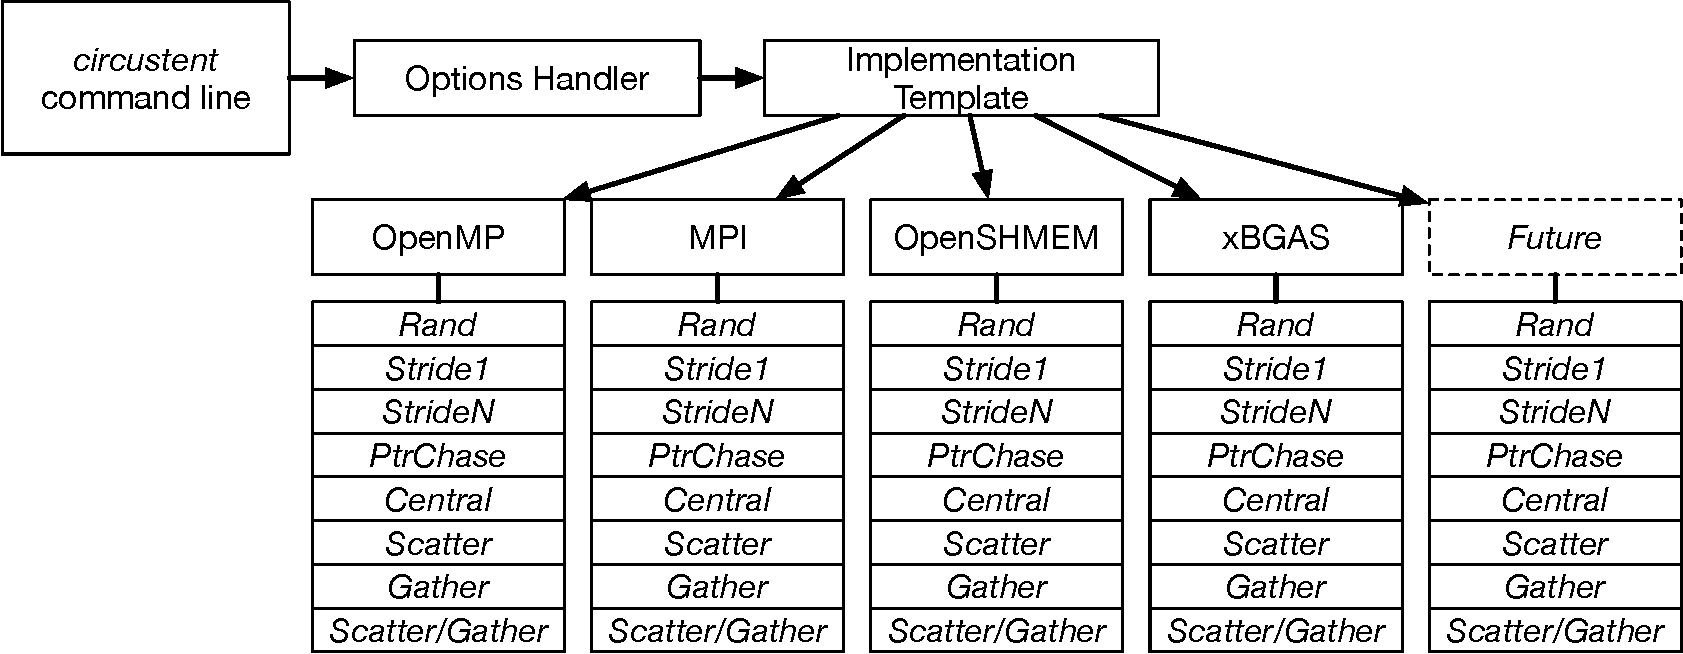
\includegraphics[width=5in]{figures/arch.pdf}
\caption{CircusTent Architecture}
\label{fig:ct_arch}
\end{figure*}

\todo[inline]{I'd suggest to classify related work into a few categories and
have a sub-section for each category to make the organization and presentation
better structured. -Yong}

Several previous studies have examined the behavior and performance characteristics of different synchronization primitives.
Villa et al. explored the efficiency and scalabilty of barrier based synchronization on manycore architectures utilizing intraprocessor interconnects modeled after the design of network-on-chip (NOC) paradigms \cite{villa2008barriers}.
In this study, the authors evaluated four different barrier algorithms, implemented in both hardware and software, using a cycle-accurate simulator.
Trials conducted using up to 128 cores, arranged in five different topologies, revealed that, at least for similar configurations, hardware based barrier implementations exhibit better performance for intraprocessor synchronization.

In a similar study, David et al. conducted an extensive investigation of synchronization that spanned multiple hardware and software methodologies \cite{david2013sync}.
Based on the results of their evaluation, the authors of this work made several important observations.
First, they note that, regardless of the implementation, synchronization across sockets is far more expensive than intrasocket synchronization.
In fact, even in the absence of contention, the authors found that the latency of operations performed on cache lines across sockets increased 2-7.5x as compared to their intrasocket analogs.
Second, they observe that the organization and behavior of the of the last-level cache (LLC) plays an important role in synchronization scalability within a socket.
Finally, they perceive that, as the number of threads contending for access to shared data grows, message-passing mechanisms often outperform locking schemes.
Overall, for physically shared memory systems such as those utilized in this work, the authors conclude that the scalability of synchronization is directly correlated to the system's architecture.

In \cite{schweizer2015evaluating}, Schweizer et al. develop a methodology for analyzing the latency and bandwidth of atomic operations.
In particular, they study the effects of different cache coherency states and complex memory hierarchies on these operations.
Using their proposed methodology, they then evaluate three different RMW atomic operations on a number of x86 platforms.
As part of this evaluation, they show that, contrary to popular belief, all of the tested atomic operations exhibit comparable performance in terms of latency and bandwidth.
Further, they find that, even in the absence of dependencies between instructions, the design of atomic operations on the tested platforms inherently prevents instruction-level parallelism.

Hoseini et al. also study the properties of atomic operations in physically shared memory systems \cite{hoseini2019modeling}.
For their investigation, they monitor accesses to shared cache lines in conditions that simulate both high and low levels of contention.
Notably, for the high contention environment, wherein requests to a single cache line become serialized, they examine the scheduling of thread accesses.
For one platform utilizing a Xeon-E5 processor, they were unable to discern any deterministic scheduling pattern.
However, for the other platform featuring a Knights Landing Xeon Phi processor, they observe that threads pinned to cores coresident on the same tile were always scheduled sequentially.
This is logical as this processor employs L2 caches that are shared between cores on the same tile, but does not include an LLC shared between all cores.

The Spatter Benchmark, developed by Lavin et al., is also directly relevant to this work \cite{lavin2018spatter}.
Although Spatter does not analyze the performance of synchronization primitives or atomic operations, similar to CircusTent, it is designed to benchmark the memory hierarchies of target architectures.
More specifically, Spatter measures an architecture's memory performance with respect to an emerging class of indexed memory access patterns known as scatter and gather operations.
Highly tunable, Spatter provides an efficient means of measuring these irregular, non-uniform memory access patterns increasingly common to HPC applications in a manner previous existing benchmarks could not.
Currently, Spatter supports both OpenMP and CUDA backend implementations for both CPU and GPGPU based platforms.
As detailed in Section \ref{subsec:algorithms}, CircusTent also integrates kernels that replicate these memory access patterns using atomic operations. 

In contrast to previous works, CircusTent, as introduced in the following section, ...

\todo[inline]{Possibly add transactional memory papers depending on space}

\todo[inline]{I'd suggest to add TM discussion please, as reviewers would expect this
discussion and a comparison when we discuss AMOs. -Yong}
